%; whizzy section -pdf xpdf -latex ./whizzypdfptex.sh
% latex beamer presentation.
% platex, latex-beamer でコンパイルすることを想定。 

%     Tokyo Debian Meeting resources
%     Copyright (C) 2008 Junichi Uekawa

%     This program is free software; you can redistribute it and/or modify
%     it under the terms of the GNU General Public License as published by
%     the Free Software Foundation; either version 2 of the License, or
%     (at your option) any later version.

%     This program is distributed in the hope that it will be useful,
%     but WITHOUT ANY WARRANTY; without even the implied warranty of
%     MERCHANTABILITY or FITNESS FOR A PARTICULAR PURPOSE.  See the
%     GNU General Public License for more details.

%     You should have received a copy of the GNU General Public License
%     along with this program; if not, write to the Free Software
%     Foundation, Inc., 51 Franklin St, Fifth Floor, Boston, MA  02110-1301 USA

\documentclass[cjk,dvipdfmx,12pt]{beamer}
\usetheme{Tokyo}
\usepackage{monthlypresentation}

%  preview (shell-command (concat "evince " (replace-regexp-in-string "tex$" "pdf"(buffer-file-name)) "&"))
%  presentation (shell-command (concat "xpdf -fullscreen " (replace-regexp-in-string "tex$" "pdf"(buffer-file-name)) "&"))

%http://www.naney.org/diki/dk/hyperref.html
%日本語EUC系環境の時
\AtBeginDvi{\special{pdf:tounicode EUC-UCS2}}
%シフトJIS系環境の時
%\AtBeginDvi{\special{pdf:tounicode 90ms-RKSJ-UCS2}}

\title{東京エリア Debian 勉強会}
\subtitle{資料}
\author{岩松 信洋 iwamatsu@debian.or.jp\\IRC nick: iwamatsu}
\date{2008年9月20日}
\logo{
\includegraphics[width=8cm]{image200607/openlogo-light.eps}}

\begin{document}

\frame{\titlepage{}}


\section{Intro}

\emtext{設営準備にご協力ください}

\begin{frame}
 \frametitle{Agenda}
\begin{minipage}[t]{0.45\hsize}
  \begin{itemize}
  \item 注意事項
	\begin{itemize}
	 \item 飲食禁止
	 \item 政治/宗教/営利活動禁止
	\end{itemize}
  \item quiz
  \item 最近のDebian関連のイベント
	\begin{itemize}
	 \item 前回の勉強会 
	\end{itemize}
 \end{itemize}
\end{minipage} 
\begin{minipage}[t]{0.45\hsize}
 \begin{itemize}
  \item Po4a でドキュメント翻訳の保守を楽にしよう
  \item 【でびあん】Debian パッケージメンテナというお仕事【現在募集中】
 \end{itemize}
\end{minipage}
\end{frame}

\section{最近}


\begin{frame}
 \frametitle{Agenda}
\begin{minipage}[t]{0.45\hsize}
  \begin{itemize}
  \item 注意事項
	\begin{itemize}
	 \item 飲食禁止
	 \item 政治/宗教/営利活動禁止
	\end{itemize}
  \item quiz
  \item 最近のDebian関連のイベント
	\begin{itemize}
	 \item 前回 
	\end{itemize}
 \end{itemize}
\end{minipage} 
\begin{minipage}[t]{0.45\hsize}
 \begin{itemize}
  \item Debconf 8
  \item Debian 温泉
  \item 第90回カーネル読書会
 \end{itemize}
\end{minipage}
\end{frame}



\section{DWN quiz}
\begin{frame}{Debian 常識クイズ}

Debian の常識、もちろん知ってますよね?
知らないなんて恥ずかしくて、知らないとは言えないあんなことやこんなこと、
みんなで確認してみましょう。

今回の出題範囲は\url{debian-devel-announce@lists.debian.org} に投稿された
内容とDebian Project Newsからです。

\end{frame}

\subsection{問題}

 \santaku
 {今年も Debconf が開催されました。どこで開催されたでしょうか。}
 {中国}
 {アルゼンチン}
 {スペイン}
 {B}
 
 \santaku
 {ギブアップ宣言をした Debian サブプロジェクト/チームは何でしょうか}
 {The Debian Live project}
 {The Debian EEEPC team}
 {The Debian Jr. project}
 {C}

 \santaku
 {Lenny frozen が宣言されたのはいつ?}
 {2008/07/26}
 {2008/07/27}
 {2008/07/28}
 {B}
 
 \santaku
 {Andreas Schuldei が立ち上げた新しいチームは何でしょうか。}
 {Debian マーケティング チーム}
 {Debian Dream チーム}
 {Debian Chrome チーム}
 {A}

 \santaku
 {Debian GNU/Linux 4.0 のアップデート版が出ましたが、何と呼ばれているでしょうか。}
 {etch and lenny}
 {etch with you}
 {etch and a half}
 {C}

 \santaku
 {リリースに向けての作業が佳境に入っています。このような作業の中、lennyの次のバージョンとなるリリースのコードネームが決まりました。何でしょうか。}
 {3つ目エイリアン squeeze}% 3つ目エイリアン
 {言葉遊びのオモチャ spell}%言葉遊びのオモチャ
 {重量挙げ選手のアクションフィギュア rocky}%重量挙げ選手のアクションフィギュア
 {A}



\section{最近のDebian関連のイベント}
\emtext{Debconf8}
\emtext{Debian温泉}
\emtext{第90回 カーネル読書会}

\section{事前課題紹介}
\emtext{事前課題の紹介}
% pre work home work

\begin{frame}{事前課題}
今回の事前課題は
\begin{enumerate}
\item Debianで気になった翻訳されていないもの
\item あなたの考えている Debian パッケージメンテナの想像図
\end{enumerate}
というものでした。
その課題に対して下記の内容を提出いただきました。
\end{frame}

\begin{frame}{前田さん}

\textbf{Debian 気になった翻訳されていないもの}\\
とりあえずよく使いそうなmanマニュアルでどのくらい翻訳されていないのかをざっと調べてみました。
\begin{itemize}
  \item 無線LAN関係のmanマニュアル
    \begin{itemize}
      \item wireless-toolsパッケージのmanマニュアル。
      \item wpa\_supplicant(8), wpa\_supplicant.conf(5)
      \item wpa\_gui(8)
    \end{itemize}

  \item セキュリティ関連ツールのmanマニュアル。
    \begin{itemize}
      \item gpg(1)
      \item openssl(1ssl) (ところでこれ、何故OPENSSL(1SSL)何でしょうかね?)
      \item tripwire(8), twadmin(8)
      \item ssh(1), sshd(8), sshd\_config(5), ssh\_config(5)
      \item bastille(1m)
      \item chkrootkit(1)
    \end{itemize}
\end{itemize}
\end{frame}

\begin{frame}
\begin{itemize}
  \item システム管理系のmanマニュアル。
    \begin{itemize}
      \item syslog-ng(8)
      \item inetd(8) (個人的にはinetdはもう使っていないですが、デフォルトでは入ってますよね)
      \item interfaces(5)
      \item logrotate(8)
      \item gshadow(5)
      \item pam(7)
      \item udev(7)
      \item vim(1)
    \end{itemize}
\end{itemize}
面倒になったので途中で調べるの止めました。
有線LANに比べると設定が面倒なので日本語になっていないと一般の人には余計に敷居が上がるだろうと思います。
ただ、無線LANとかセキュリティ関連(特にOpenSSHとか)は、Upstreamの更新頻度&一度の変更での差異が大きいのも原因でしょうか。\\
やることいっぱいありますね…。

\end{frame}

\begin{frame}
\begin{itemize}
  \item システム管理系のmanマニュアル。
    \begin{itemize}
      \item syslog-ng(8)
      \item inetd(8) (個人的にはinetdはもう使っていないですが、デフォルトでは入ってますよね)
      \item interfaces(5)
      \item logrotate(8)
      \item gshadow(5)
      \item pam(7)
      \item udev(7)
      \item vim(1)
    \end{itemize}
\end{itemize}
面倒になったので途中で調べるの止めました。
有線LANに比べると設定が面倒なので日本語になっていないと一般の人には余計に敷居が上がるだろうと思います。
ただ、無線LANとかセキュリティ関連(特にOpenSSHとか)は、Upstreamの更新頻度&一度の変更での差異が大きいのも原因でしょうか。
やることいっぱいありますが、\textbf{しょうがないので全部翻訳する予定です。}

\end{frame}

\begin{frame}{平澤さん}
\textbf{私の考えるDebian パッケージメンテナの想像図}\\
ほんとに想像でしかかけないのですが..........
お題を3つの単語にわけてみて、想像をふくらましてみます。

まず、{\bf Debian} について。安定性を重視したディストリビューションと聞いている。

きっと、Debianの裏方(メンテナー?)さんが
ライブラリなどの依存関係なんかを細かく確認をしながら
リリースするんだろうなぁ、とか想像する。

次、{\bf パッケージ}. 個別のプログラムをxxx.debファイルにまとめられている状
態を指す?
それとも {\bf current}、{\bf stable}, {\bf testing}と呼ばれている、カテゴリー分けされ
たプログラムの
塊のことを指すのかしら? よくわからない。
\end{frame}

\begin{frame}
次、{\bf メンテナ}. 訳するとメンテナンスをする人
想像が想像をよび、すでに妄想の状態かも。

いい仕事をする {\bf 仕事人}のことを指すのでしょうか?
仕事の一部は定型化されていると想像するので、ルーチンワーク
な部分をやっつけるツールってのがたくさんあるんだろうな?とか想像。
\end{frame}

\begin{frame}{やまねさん}
\textbf{Debian で気になった翻訳されていないものを教えてください}\\
gkstu, update-manager (すいません、まだやってませんでした…)

\end{frame}

\begin{frame}{やまねさん}
\textbf{Debian で気になった翻訳されていないものを教えてください}\\
gkstu, update-manager (すいません、まだやってませんでした…)
\textbf{なので、頑張って po-debconf を全部翻訳します。}
\end{frame}

\begin{frame}{山本さん}
\textbf{Debian で気になった翻訳されていないものを教えてください}\\
\url{http://www.debian.org} の文書は大体翻訳されてきたと思うけど、
最近は \url{http://wiki.debian.org} で盛んに文書が出されたり、
編集されたりしてるよね。

特に lenny でリリース予定(だっけ?)の armel のページなんかは
\url{http://www.debian.org/ports} から wiki へのリンクぐらいしかない。
当然、翻訳なんかもないが、そろそろなんとかねにゃいかん気もする。
\url{http://wiki.debian.org} で気になるのは、まだまだあるんじゃないかな?
\end{frame}

\begin{frame}{山本さん}
\textbf{Debian で気になった翻訳されていないものを教えてください}\\
\url{http://www.debian.org} の文書は大体翻訳されてきたと思うけど、
最近は \url{http://wiki.debian.org} で盛んに文書が出されたり、
編集されたりしてるよね。

特に lenny でリリース予定(だっけ?)の armel のページなんかは
\url{http://www.debian.org/ports} から wiki へのリンクぐらいしかない。
当然、翻訳なんかもないが、そろそろなんとかねにゃいかん気もする。
\url{http://wiki.debian.org} で気になるのは、まだまだあるんじゃないかな?
\textbf{なので全部翻訳します。}
\end{frame}

\begin{frame}
\textbf{あなたの考えている Debian パッケージメンテナの想像図}\\
きっと、スーパーなハカーに違いない!
コーラとピザを片手に、コードを書いているんだ!
\end{frame}

\begin{frame}
\textbf{あなたの考えている Debian パッケージメンテナの想像図}\\
きっと、スーパーなハカーに違いない!
コーラとピザを片手に、コードを書いているんだ!
\begin{center}
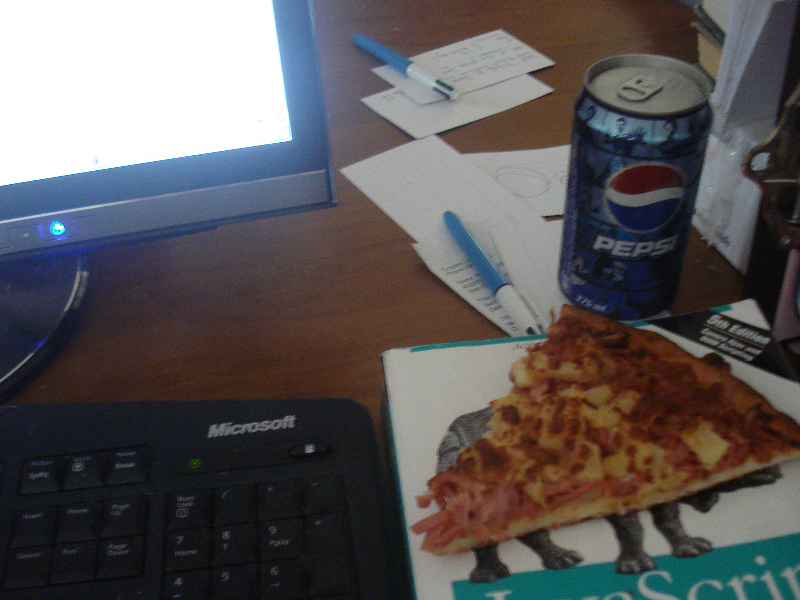
\includegraphics[width=10cm]{image200809/hack-pizza.png}
\end{center}
\end{frame}

\begin{frame}{つじかたさん}
\textbf{Debianで気になった翻訳されていないものを教えてください}\\
CDBSのドキュメント。
以前、CDBSを勉強しようと思ったのですが、日本語ドキュメントが見つからず挫折しました。
今、「入門Debianパッケージ」読んで勉強してます。
\end{frame}


\begin{frame}{つじかたさん}
\textbf{Debianで気になった翻訳されていないものを教えてください}\\
CDBSのドキュメント。
以前、CDBSを勉強しようと思ったのですが、日本語ドキュメントが見つからず挫折しました。
今、「入門Debianパッケージ」読んで勉強してます。
\textbf{けど、CDBSを日本語で読みたいので、翻訳してみます。}
\end{frame}

\begin{frame}{吉田@板橋さん}
\textbf{Debian パッケージメンテナの想像図}\\
\textbf{編集者により削除されました。}

\textbf{Debian で気になった翻訳されていないものを教えてください}\\
lintianのメッセージ、aptのman,gpgのman。
lintianのメッセージの対処方法(黙らせ方)がぐぐっても、
翻訳サイトに掛けても良くわからない。
日本語にすればわかるのか?といえばそれも微妙だが。
aptitudeのmanは日本語化されているのにaptのmanは日本語化されていない
ぐ(以下略)しても太古のMLの断片が出てくるだけ...
gpg(GnuPG)の日本語man...ぐ(略、現状地球上になさげ。訳してみようと思ったが、
量が多すぎて挫折。
\end{frame}


\begin{frame}{吉田@板橋さん}
\textbf{Debian パッケージメンテナの想像図}\\
\textbf{編集者により削除されました。}

\textbf{Debian で気になった翻訳されていないものを教えてください}\\
lintianのメッセージ、aptのman,gpgのman。
lintianのメッセージの対処方法(黙らせ方)がぐぐっても、
翻訳サイトに掛けても良くわからない。
日本語にすればわかるのか?といえばそれも微妙だが。
aptitudeのmanは日本語化されているのにaptのmanは日本語化されていない
ぐ(以下略)しても太古のMLの断片が出てくるだけ...
gpg(GnuPG)の日本語man...ぐ(略、現状地球上になさげ。訳してみようと思ったが、
量が多すぎて挫折。
\textbf{が、手元のHDDからサルベージに成功した気がしたので、再度頑張ります。}
\end{frame}

\begin{frame}{たかはし あきゆき さん}
\textbf{Debian パッケージメンテナの想像図}
俺はプログラムなんて書けないけど」が口癖の黒魔術士

\textbf{Debian で気になった翻訳されていないものを教えてください}\\
lennyのアップデート・マネージャが気になります。
\end{frame}

\begin{frame}{たかはし あきゆき さん}
\textbf{Debian パッケージメンテナの想像図}\\
俺はプログラムなんて書けないけど」が口癖の黒魔術士

\textbf{Debian で気になった翻訳されていないものを教えてください}\\
\textbf{lennyのアップデート・マネージャが気になったので翻訳します。}
\end{frame}

\begin{frame}{あけどさん}
\textbf{Debian で気になった翻訳されていないものを教えてください}\\
DebianというかUpstreamになるかと思うのですが、rubyやperlのマニュアルページは未だ日本語版が無いようです。
マニュアルページでは他にも日本語版の無い物が色々とありますね。
それと、翻訳とはちょっと違うのですが
\url{http://manpages.debian.net/} で提供されている日本語版のページで文字化けが気になる所です。
Debian関係では、Debian Wiki の日本語化の残っている所がまだまだありますし、
WebドキュメントのDebian Developer's Referenceの日本語ページが
去年から手を着けたまま未完了なのが気になっています。(査読をお手伝い途中のままですみません。)
\end{frame}

\begin{frame}{あけどさん}
\textbf{Debian で気になった翻訳されていないものを教えてください}\\
DebianというかUpstreamになるかと思うのですが、rubyやperlのマニュアルページは未だ日本語版が無いようです。
マニュアルページでは他にも日本語版の無い物が色々とありますね。
それと、翻訳とはちょっと違うのですが
\url{http://manpages.debian.net/} で提供されている日本語版のページで文字化けが気になる所です。
Debian関係では、Debian Wiki の日本語化の残っている所がまだまだありますし、
WebドキュメントのDebian Developer's Referenceの日本語ページが
去年から手を着けたまま未完了なのが気になっていますが、\textbf{男なので最後までやり遂げる次第です。}

\end{frame}

\begin{frame}
\textbf{あなたの考えている Debian パッケージメンテナの想像図}\\
具体的な人物が思いつくので想像というよりそのものって感じでしょうか。
なので、詳細については控えさせて頂きたく存じます。
\end{frame}

\begin{frame}
\textbf{あなたの考えている Debian パッケージメンテナの想像図}\\
具体的な人物が思いつくので想像というよりそのものって感じでしょうか。
なので、詳細については控えさせて頂きたく存じます。
\begin{center}
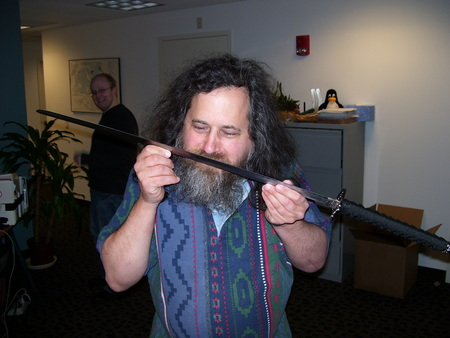
\includegraphics[width=10cm]{image200809/rms_katana.jpg}
\end{center}
\end{frame}

\begin{frame}{hidewon さん}
\textbf{あなたの考えている Debian パッケージメンテナの想像図}\\
いつもパソコンの画面の前に座り、ジャンク
フードを食しながら、あらゆるUNIXコマンドを
あやつり、それらの結果に一喜一憂をし、液晶画面を
みながら明日のソフトウェアを創造しつづけるスーパーハッカー。
とてもすごいひとたち。

パッケージの依存を解決したり、バグが発見されれ
ばそれらを瞬時に解決しなければならないのでしょうか。
英語のパッケージである場合、それらは英語で
作者に問い合わせるなどの折衝役もしなければ
ならないのでしょうか。パッケージが書かれている
言語がじぶんのしらないもので書かれている場合、
それらを自分でなんとかしなければならないのでしょうか。
あるいは修正できるスキルがなければメンテナンスを
してはいけないのでしょうか。プログラミングの経験は
必須なのでしょうか。いったいどんな作業がおこなわれて
いるのか知りたいです。
\end{frame}

\begin{frame}
こんなこととか、
\begin{center}
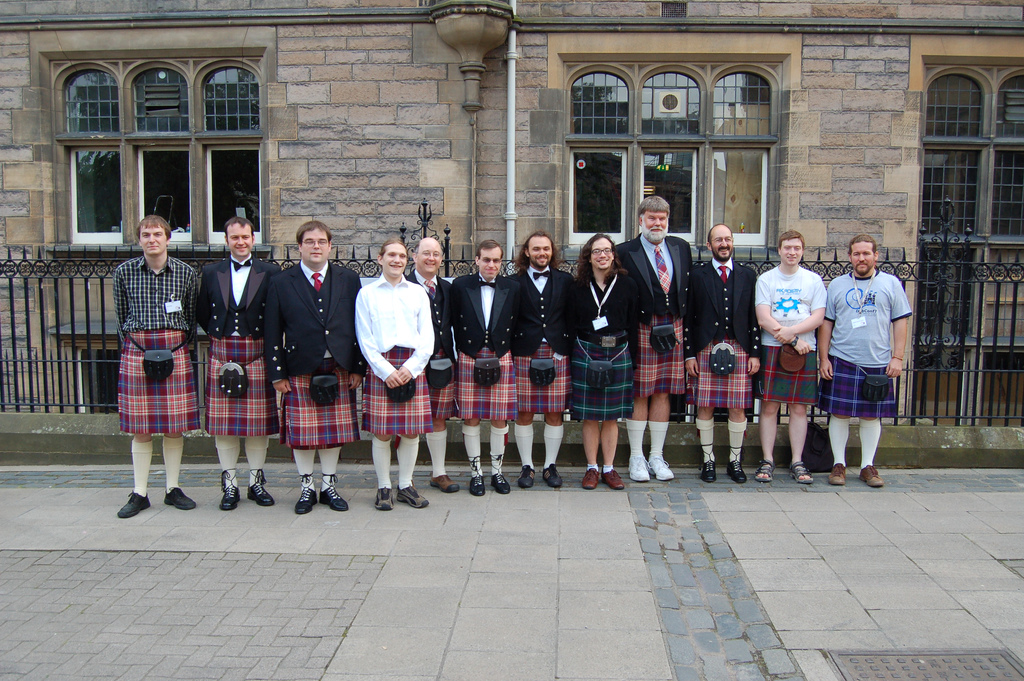
\includegraphics[width=12cm]{image200809/debconf7-member.jpg}
\end{center}
\end{frame}

\begin{frame}
こんなことをしています。
\begin{center}
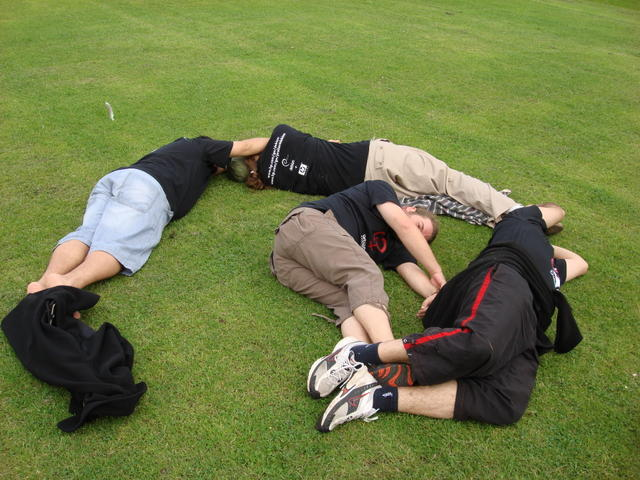
\includegraphics[width=12cm]{image200809/guru.jpg}
\end{center}
\end{frame}

\begin{frame}
ときどきソフトウェアの不具合などがあるとき、パッケージを
展開すると知らないひとのなまえとメールアドレスがありました。
あれがメンテナでしょうか。そうだとすればあれがぼくと彼らを
つなぐ唯一の接点でした。
ここへ連絡をとってしまっていいものだろうか?となやむことが
よくあります。メンテナというひとがどんなひとでどんなことを
しているひとなのかということがわからないので、連絡をとるのが
怖かったのです。

メンテナはどんなひとたちでしょうか。
\end{frame}

\begin{frame}
こんな人たちです。
\begin{center}
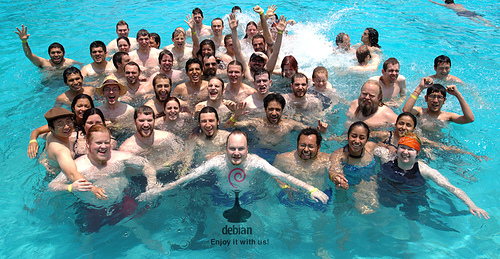
\includegraphics[width=12cm]{image200809/debian-swim.jpg}
\end{center}
\end{frame}

\begin{frame}{森田 尚さん}
\textbf{Debianで気になった翻訳されていないもの}\\
自分が知らないだけかもしれませんが、
\begin{itemize}
  \item jargon - the definitive compendium of hacker slang
  \item fortunes - Data files containing fortune cookies
\end{itemize}
とか。
\end{frame}

\begin{frame}{森田 尚さん}
\textbf{Debianで気になった翻訳されていないもの}\\
自分が知らないだけかもしれませんが、
\begin{itemize}
  \item jargon - the definitive compendium of hacker slang
  \item fortunes - Data files containing fortune cookies
\end{itemize}
とか\textbf{が気になったので翻訳してみます。}
\end{frame}

\begin{frame}{キタハラ さん}
\textbf{Debianで気になった翻訳されていないものを教えてください}\\
{\bf Etch} のGUIインストールをした時に説明文
の中で日本語になってい無い所があったのを思い出した
が、どこだったが思い出せない。 当時のメモを見ると
{\bf uswsusp}の説明が英語で迷った」とあるのでこれ
だと思うが、これを見てもまだ思い出せない。 最近、
いろんな事がありすぎたせいか、歳のせいか?
\end{frame}

\begin{frame}{キタハラ さん}
\textbf{Debianで気になった翻訳されていないものを教えてください}\\
{\bf Etch} のGUIインストールをした時に説明文
の中で日本語になってい無い所があったのを思い出した
が、どこだったが思い出せない。 当時のメモを見ると
{\bf uswsusp}の説明が英語で迷った」とあるのでこれ
だと思うが、これを見てもまだ思い出せない。 最近、
いろんな事がありすぎたせいか、歳のせいか
\textbf{と思いましたが、気のせいだったので翻訳してみます。}
\end{frame}


\begin{frame}{日比野 さん}
\textbf{Debianで気になった翻訳されていないものを教えてください}\\

私の場合のお約束ということで関数型言語系を挙げておきます。
Developing Applications With Objective Camlという
原著がフランス語のOCamlの本の英訳が ocaml-book-en というパッケージにあります。
その英訳がさらに日本語になると嬉しいなあとか。
途中までは \url{http://d.hatena.ne.jp/sumii/20060408/1144492539} に有ったりしますが。
\end{frame}


\begin{frame}{日比野 さん}
\textbf{Debianで気になった翻訳されていないものを教えてください}\\

私の場合のお約束ということで関数型言語系を挙げておきます。
Developing Applications With Objective Camlという
原著がフランス語のOCamlの本の英訳が ocaml-book-en というパッケージにあります。
その英訳がさらに日本語になると嬉しいなあとか。
途中までは \url{http://d.hatena.ne.jp/sumii/20060408/1144492539} に有ったりしますが、
\textbf{私が追従してフランス語から日本語にします。}
\end{frame}

\begin{frame}{岩松}
\textbf{Debianで気になった翻訳されていないものを教えてください}\\
Git, Xfce 全般、awesome

\textbf{あなたの考えている Debian パッケージメンテナの想像図}\\
ツンデレ。
\end{frame}


% (query-replace "\\subsection" "\\end{frame}\\begin{frame}")
% (query-replace "\\subsubsection" "\\textbf")


% (query-replace "\\subsection" "\\end{frame}\\begin{frame}")
% (query-replace "\\subsubsection" "\\textbf")


\emtext{2008年計画}

\begin{frame}{2008年計画}

{\scriptsize
\begin{enumerate}
 \item 新年会「気合を入れる」
 \item Open Source Conference Tokyo (3/1)
 \item データだけのパッケージを作成してみる、
       ライセンスの考え方 (David Smith)
 \item バイナリ一つのパッケージを作成してみる (吉田@板橋)\\
       バージョン管理ツールを使いDebianパッケージを管理する(git)\\
       アップストリームの扱い(svn/git/cvs)(岩松 信洋さん)
 \item バイナリの分けたパッケージの作成。(前田さん)\\
       バイナリの分け方の考え方、アップグレードなどの運用とか。
 \item パッケージ作成(dpatch/debhelperで作成するパッケージ)(小林儀匡さん)\\
       man の書き方(roff or docbook)(でんさん)\\
       Open Source Conference Hokkaido
 \item パッケージ作成(kernel patch、kernel module)
       、Debconf発表練習
 \item Debconf アルゼンチン、Debian温泉

 \item Open Source Conference Tokyo/Fall、
       デーモン系のパッケージの作成、latex、 emacs-lisp、フォントパッケージ
 \item パッケージの cross-compile の方法、amd64 上で i386 のパッケージと
       か、OSC-Fall報告会、Debconf報告会
 \item 国際化 po-debconf / po化 / DDTP
 \item 忘年会
\end{enumerate}
}
\end{frame}
\emtext{【でびあん】Debian パッケージメンテナというお仕事【現在募集中】}
\emtext{Po4a でドキュメント翻訳の保守を楽にしよう}

\emtext{次回の勉強会}
\begin{frame}{次回の勉強会}
次回の勉強会は OSC 2008 Tokyo Fall です。
\begin{itemize}
 \item セミナー: 「あなた」とオープンソース/フリーソフトウェア、そして「Debian」

「オープンソース/フリーソフトウェアは、「あなた」にとってどんな価値があるのでしょうか?どのような利益をもたらすものなのでしょうか?不利益は生じないのでしょうか?「自由」を求めるディストリビューション Debian のパッケージメンテナの一人として、そして個人/会社等での利用者としてこれらに接する立場から改めて考えた視点を伝えます。」

と、やまねさんが語ります。
\end{itemize}
\end{frame}

\begin{frame}
\begin{itemize}
 \item ミニセミナー:Debian でぶっこぬき! FLOSS のみでつくる Flash 再生環境

「自由なソフトウェアのみで構成される Debian GNU/Linux。プロプラエタリなソフトウェアの代表である flash-plugin を使わずに GNU/Linux 上で生き延びる方法を話すかもしれません。」

と岩松が語るかもしれません。

\item パネルディスカッション : 勉強会大集合

東京エリアDebian勉強会の運営方法とバッドノウハウについて、岩松が熱く語るかもしれません。

\item 展示\\
 Debianマシン、勉強会資料の展示、フライヤーおよびインストールCDの配布を行います。
\end{itemize}
\end{frame}

\begin{frame}{宴会場所}
\begin{itemize}
 \item 宴会場所\\
       本日の宴会は「庄屋」です。\\
       参加者はフロアに集合し、全員で移動しましょう。やまもとさんが幹事です。
 \item 片付け\\
       部屋を片付けるのにご協力ください。
\end{itemize}

\end{frame}

\begin{frame}{利用した画像}
\begin{itemize}
\item pizza の画像 (C)bootload\\
\url{http://flickr.com/photos/bootload/2648255609/}
\item RMS の画像 (C)Alejandro Santos
\url{http://www.alejolp.com/blog/wp-content/uploads/2007/04/rms_katana.jpg}
\item Second Debconf 6 pool group photo(debian-swim.jpg) (c) aigarius
\url{http://flickr.com/photos/aigarius/542611481/}
\item debconf7-member.jpg (C) Wouter Verhelst
\url{http://flickr.com/photos/53246655@N00/581894457}
\item It does look like a Debian swirl :) (guru.jpg)
\url{https://gallery.debconf.org/v/debconf7/album18/dsc00944.jpg.html}
\end{itemize}

\end{frame}

\end{document}

;;; Local Variables: ***
;;; outline-regexp: "\\([ 	]*\\\\\\(documentstyle\\|documentclass\\|emtext\\|section\\|begin{frame}\\)\\*?[ 	]*[[{]\\|[]+\\)" ***
;;; End: ***
